\documentclass[pdflatex,landscape,titlepage]{foils}
\usepackage{graphicx,natbib}
\usepackage{setspace}
\usepackage{pause}
\usepackage[bgadd]{background}
\usepackage{mpmulti}
\usepackage{pp4slide}
\usepackage{booktabs}
\usepackage{amsmath}
\usepackage{pdf14}


% === dcolumn package ===
\usepackage{dcolumn}
\newcolumntype{.}{D{.}{.}{-1}}
\newcolumntype{d}[1]{D{.}{.}{#1}}

%Check if we are compiling under latex or pdflatex
\ifx\pdftexversion\undefined
  \usepackage[dvips]{graphics}
\else
  \usepackage[pdftex]{graphics}
\fi


%% hyperref options
\usepackage[bookmarksopen]{hyperref}
\hypersetup{%
  pdftitle = { } 
  pdfsubject = {}
  pdfauthor = {}
}


%% definecolor
\usepackage{color}
\renewcommand\normalcolor{\color{white}} % Color of the text of \foilhead{}
\pagecolor{black}
\color{white}

\tolerance = 1500

\addtolength{\hoffset}{-0.6in} 
\addtolength{\voffset}{-1in}
\addtolength{\textwidth}{1.2in} 
\addtolength{\textheight}{2in}

\definecolor{black1}{rgb}{0,0,0}
\definecolor{blue1}{rgb}{0,0,.8}
\renewcommand\normalcolor{\color{green}} % Color of the text of \foilhead{}
\color{white}


\title{{\large \textcolor{green}{POLS/CSSS 503: \\
Advanced Quantitative Political Methodology}} \\
\vspace{.75in}
Introduction to the Course \& to R
\vspace{.5in}
}
\author{\textsf{\large Christopher Adolph}\\\vspace{1 em}\\{ 
\textsf{\small Department of Political Science} \\ \vspace{0.5em} \emph{\textsf{\small and}} \\ \vspace{0.0em} \textsf{\small Center for Statistics and the
Social Sciences} \\ \vspace{0.5em}
  \textsf{\small University of Washington, Seattle}}}

\date{}
\begin{document}

\vpagecolor[blue1]{black1}

\maketitle
\pagestyle{empty}
\clearpage

\foilhead[-0.75in]{POLS 503 Course Goals}
\bgclear

Course Goals:

\begin{enumerate}

\item Learn the properties and limitations of the linear regression model

\item Develop further skills in interpreting \& fitting linear models

\item Study extensions of the linear model to deal with common problems

\item Become comfortable with matrix algebra representions of models

\item Gain proficiency in \texttt{R}, a powerful and popular statistical package

\item Get ready to take POLS/CSSS 510: MLE,  or other advanced CSSS courses

\end{enumerate}

\foilhead[-0.75in]{Agenda for this week}
\bgclear

\begin{itemize}
\item Introductory example:  why focus on model interpretation?

\item Overview of syllabus \& course requirements

\item Introduction to R
\end{itemize}


\foilhead[-0.75in]{How do we intrepret our models?}
\bgclear

For simple versions of linear regression,\\ coefficients \&
se's usefully summarize the relation between $x$ and $y$

But how do we interpret $\beta$ when we add to the linear regression model\ldots

\begin{itemize}
\item transformed variables? \pause \quad 
  \color{green} $\mathrm{log}(\mathrm{income}) = \alpha +
  \beta_1\mathrm{age} + \varepsilon$  \pause

\quad \quad \quad \quad \quad  \quad \quad 
 \quad \quad \quad \quad \quad \quad \quad \quad \emph{or} 

 \quad \quad \quad \quad \quad  \quad \quad 
 \quad \quad \quad \quad $\mathrm{wealth} = \alpha + \beta_2\mathrm{age}+ \beta_3\mathrm{age}^2 + \varepsilon$
 \color{white} \pause

\item interactions? \pause \quad  \color{green}
  $\mathrm{deficit} = \alpha + \beta_4\mathrm{ideology} + \beta_5\mathrm{power} + \beta_6(\mathrm{ideology} \times
  \mathrm{power}) + \varepsilon$  \color{white} \pause

\item time series dynamics? \pause \quad  \color{green}
  $\mathrm{budget}_{t} = \alpha + \beta_7\mathrm{budget}_{t-1} +
  \beta_8\mathrm{partisan}_t + \varepsilon_t$  \color{white} \pause

\item multiple equations? \pause \quad  \color{green} $\mathrm{spend} =
  \alpha + \beta_9\mathrm{compete} + \varepsilon$ \quad \pause

\quad \quad \quad \quad \quad  \quad \quad 
 \quad \quad \quad \quad \quad \quad \quad \quad\emph{and}
 
\quad \quad
  \quad \quad \quad  \quad \quad 
  \quad \quad 
  \quad $\mathrm{compete} = \eta + 
  \beta_{10}\mathrm{spend} + \nu$  \color{white} \pause

\item non-linear models? \pause \quad  \color{green} $\mathrm{Pr(war)}
  = (1 - \mathrm{exp}(-\alpha -\beta_{11}\mathrm{distance}))^{-1}$
  \color{white} 
\end{itemize}

\foilhead[-0.75in]{How do we intrepret our models?}
\bgclear

As models get more complicated, \\
learning to effectively interpret and present them gets more important

Model coefficients are not always easy to interpret

Focus on coefficients alone risks:

\begin{itemize}
\item your work being ignored or misunderstood by those who don't know the model

\item misunderstanding our own models

\item Failing to draw out all the relevant implications of the model
\end{itemize}

Graphics usually do a better job of explaining and exploring
regression models

A famous ``simple'' example shows this well

\foilhead[-0.75in]{The \emph{Challenger} launch decision}

\color{black}
\begin{center}
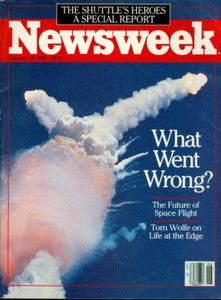
\includegraphics[width=9.5 in,,angle=180]{shuttle}
\end{center}
\color{white}

In 1986, the Challenger space shuttle exploded moments after liftoff

Decision to launch one other most scrutinized in history

Failure of O-rings in the solid-fuel rocket boosters blamed for explosion

Could this failure have been foreseen?  

\foilhead[-0.75in]{The \emph{Challenger} launch decision}

\begin{center}
\begin{tabular}{cc}
\toprule
\multicolumn{2}{c}{Flights with O-ring damage}\\
Flt Number      &       Temp (F)        \\
\midrule
2       &       70      \\
41b     &       57      \\
41c     &       63      \\
41d     &       70      \\
51c     &       53      \\
61a     &       79      \\
61c     &       58      \\
\bottomrule
\end{tabular}
\end{center}

Morton-Thiokol engineers made this table \& worried about launching below 53 degrees (Why?)

O-ring would erode or have ``blow-by'' (2 ways to fail) in cold temp

Failed to convince administrators there was a danger

(Counter-argument:  ``damages at low and high temps'')

Are there problems with this presentation?  with the use of data?

\foilhead[-0.75in]{The \emph{Challenger} launch decision}

Engineerrs did not consider successes, only failures; \\
selection on the dependent variable

\begin{center}
\begin{tabular}{ccccc}
\toprule
\multicolumn{5}{c}{All flights, chronological order}\\
Damage? &       Temp (F)        &      \quad \quad \quad        &       Damage? &       Temp (F)        \\
\midrule
No      &       66      &               &       No      &       78      \\
\color{red}\textbf{Yes}    &     \color{red}  70      &               &       No      &       67      \\
No      &       69      &               &     \color{red}   \textbf{Yes}    & \color{red}       53      \\
No      &       68      &               &       No      &       67      \\
No      &       67      &               &       No      &       75      \\
No      &       72      &               &       No      &       70      \\
No      &       73      &               &       No      &       81      \\
No      &       70      &               &       No      &       76      \\
\color{red} \textbf{Yes}    &   \color{red}     57      &               &       \color{red} \textbf{Yes}    &   \color{red}     79      \\
\color{red} \textbf{Yes}    &   \color{red}     63      &               &       No      &       76      \\
\color{red} \textbf{Yes}    &   \color{red}     70      &               &       \color{red} \textbf{Yes}    &   \color{red}     58      \\
\bottomrule
\end{tabular}
\end{center}

Other problems?  \pause Why sort by launch number?

\foilhead[-0.75in]{The \emph{Challenger} launch decision}

\begin{center}
\begin{tabular}{ccccc}
\toprule
\multicolumn{5}{c}{O-ring damage pre-Challenger, by temperature at launch}\\
Damage? &       Temp (F)        &       &       Damage? &       Temp (F)        \\
\midrule
\color{red} \textbf{Yes}        &       \color{red} 53  & \quad\quad\quad& \color{red} \textbf{Yes}     &       \color{red}70   \\
\color{red} \textbf{Yes}        &       \color{red}57   &       &       No       &       70      \\
\color{red} \textbf{Yes}        &       \color{red}58   &       &       No       &       70      \\
\color{red} \textbf{Yes}        &       \color{red}63   &       &       No       &       72      \\
No       &       66      &       &       No       &       73      \\
No       &       67      &       &       No       &       75      \\
No       &       67      &       &       No       &       76      \\
No       &       67      &       &       No       &       76      \\
No       &       68      &       &       No       &       78      \\
No       &       69      &       &       \color{red} \textbf{Yes}        &       \color{red}79   \\
\color{red} \textbf{Yes}        &       \color{red}70   &       &       No       &       81      \\
\bottomrule
\end{tabular}
\end{center}

The evidence begins to speak for itself.

What if Morton-Thiokol engineers had made this table before the launch?

\foilhead[-0.75in]{The \emph{Challenger} launch decision}

Why didn't NASA make the right decision?

Many answers in the literature:  \\
bureaucratic politics; group think; bounded rationality, etc.

But Edward Tufte thinks it may have been a matter of presentation \& modeling:

\begin{itemize}
\item Never made the right tables or graphics

\item Selected only failure data

\item Never considered a simple statistical model

\end{itemize}

What do you think?  How would you approach the data?

\foilhead[-0.75in]{The \emph{Challenger} launch decision}
\bgadd{\vspace{2.9 in} \\ 
\includegraphics[width=12 in,height=5.4 in]{whiteback.jpg}}

How about a scatterplot?  Better for seeing relationships than a table

Vertical axis is an O-ring damage index (due to Tufte, who made the plot)

\color{black}
\begin{center}
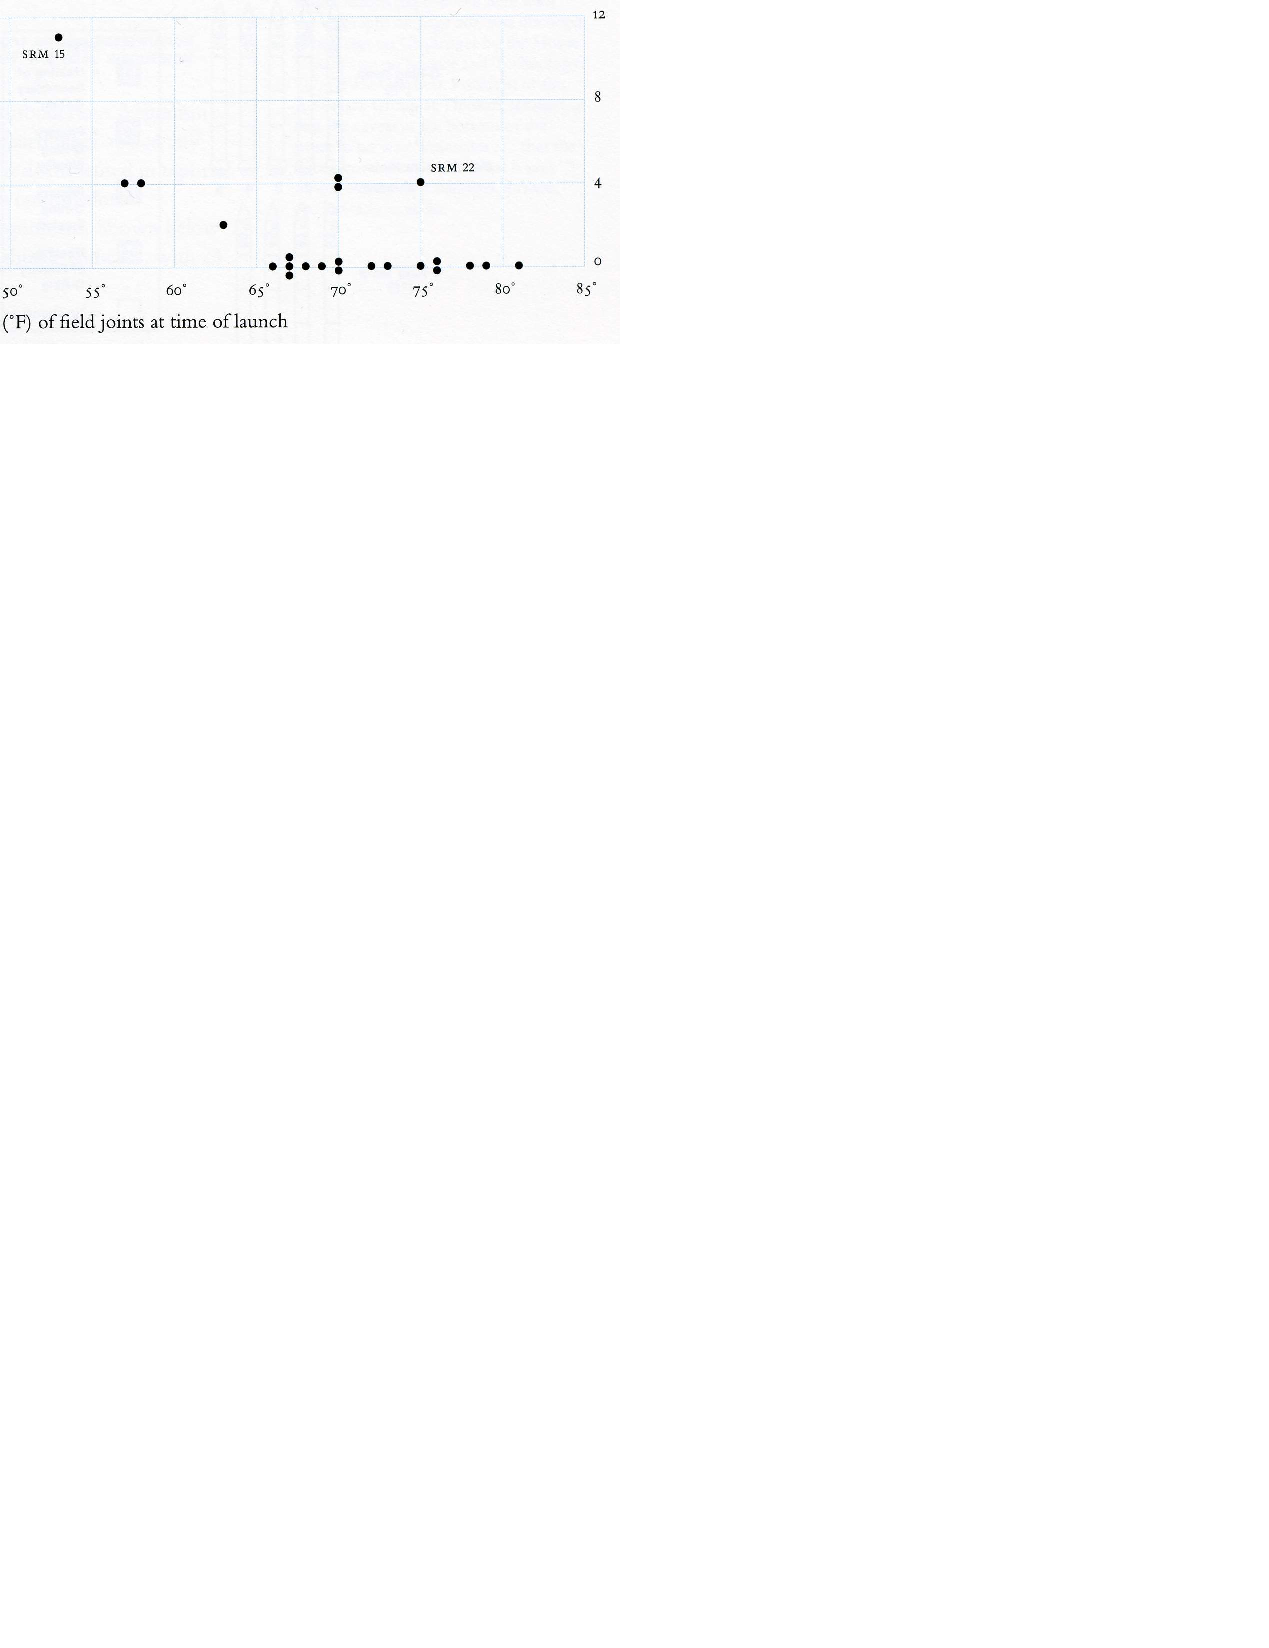
\includegraphics[width=9.5 in]{tufte_challenger_1}
\end{center}
\color{white}

Suspicious.  What the forecast temperature for launch?  

\foilhead[-0.75in]{The \emph{Challenger} launch decision}
\bgclear

What the forecast temperature for launch?

\foilhead[-0.75in]{The \emph{Challenger} launch decision}
\bgadd{\vspace{2.3 in} \\ 
\includegraphics[width=12 in,height=4.7 in]{whiteback.jpg}}

What the forecast temperature for launch?  26 to 29 degrees Fahrenheit!

\color{black}
\begin{center}
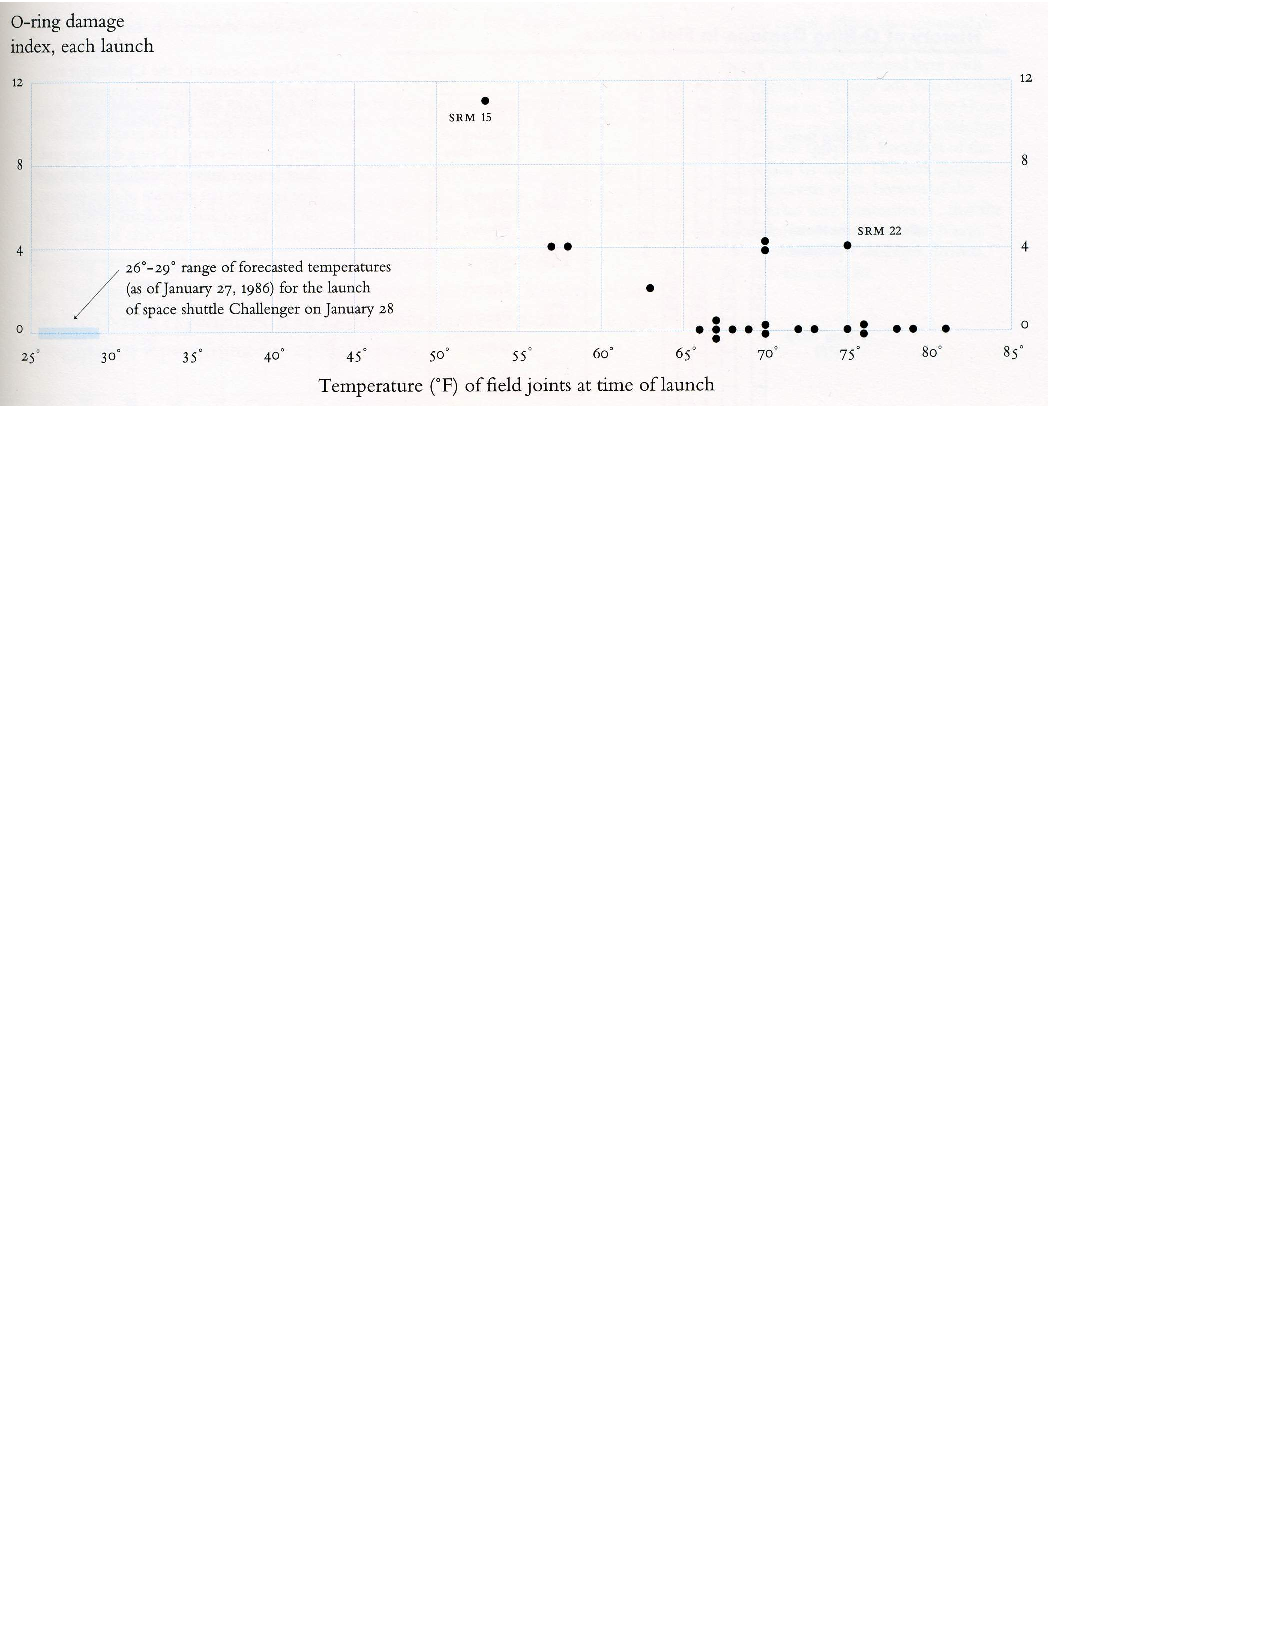
\includegraphics[width=10.5 in]{tufte_challenger_2}
\end{center}
\color{white}

The shuttle was launched in unprecendented cold

\foilhead[-0.75in]{The \emph{Challenger} launch decision}
\bgclear

Imagine you are the analyst making the launch recommendation.

You've made the scatterplot above.  What would you add to it?

Put another way, what do you is the first question you expect from your boss? \pause

``What's the chance of failure at 26 degrees?''

The scatterplot suggests the answer is ``high'', but that's vague.

But what if the next launch is at 58 degrees?  Or 67 degrees?

Clearly, we want a more precise way to state the probability of failure

We need a \emph{model}, and a way to convey that model to the public.

\foilhead[-0.75in]{The \emph{Challenger} launch decision}

A simple exercise is to model the probability of O-ring damage\\
as a function of temperature

We can use a statistical tool called ``logit'' for this purpose 

The model is nonlinear: \quad  $\mathrm{Pr(damage)}
  = (1 - \mathrm{exp}(-\beta_0 -\beta_1\mathrm{temperature}))^{-1}$ \pause

\texttt{R} gives us this lovely logit output\ldots

\begin{center}
\begin{tabular}{l...}
\toprule
Variable  &   \multicolumn{1}{c}{est.}   &   \multicolumn{1}{c}{s.e.}   &  \multicolumn{1}{c}{$p$} \\
\midrule
Temperature (F)  &  -0.18 &  0.09  & 0.047 \\
Constant     &  11.9&  6.34 &  0.062 \\
\midrule
$N$            &  22 & & \\
log-likelihood & -10.9 & & \\
\bottomrule
\end{tabular}
\end{center}

which most social scientists read as ``a statistically significant negative relationship b/w temperature and probability of damage''

But that's pretty vague too.

Is there a more persuasive/clear/useful way to present these results?


\foilhead[-0.75in]{}
\bgclear
\bgadd{\vspace{0 in} \\ 
\includegraphics[width=12 in,height=12 in]{whiteback.jpg}}

\color{black}
\begin{center}
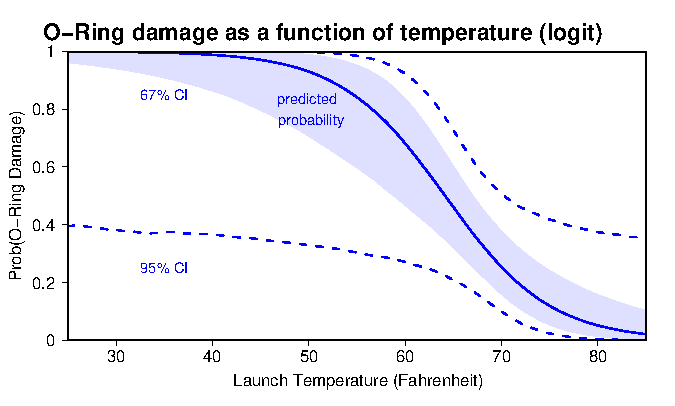
\includegraphics[width=10.5 in]{chall1}
\end{center}

A picture clearly shows non-linear model predictions \emph{and} uncertainty

\foilhead[-0.75in]{}

\color{black}
\begin{center}
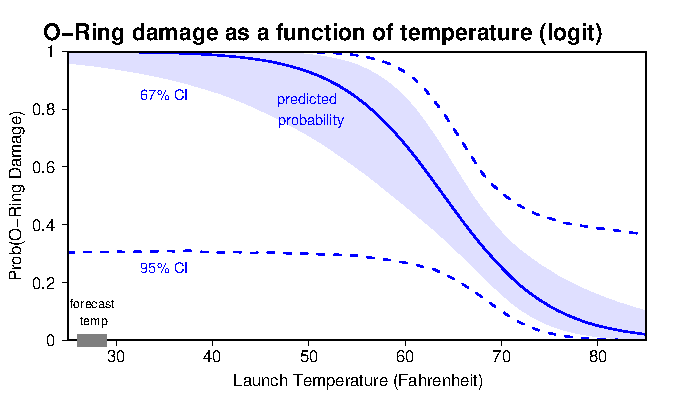
\includegraphics[width=10.5 in]{chall2}
\end{center}

And gives a more precise sense of how foolhardy launching at 29 F is.

\foilhead[-0.75in]{}

\color{black}
\begin{center}
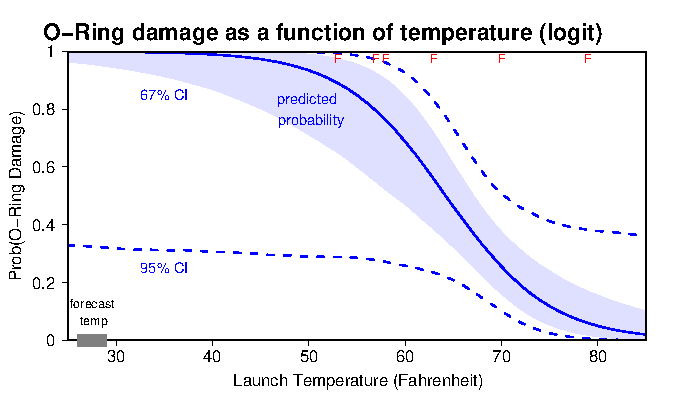
\includegraphics[width=10.5 in]{chall3}
\end{center}

It's also good to show the data giving rise to the model.

\foilhead[-0.75in]{}

\color{black}
\begin{center}
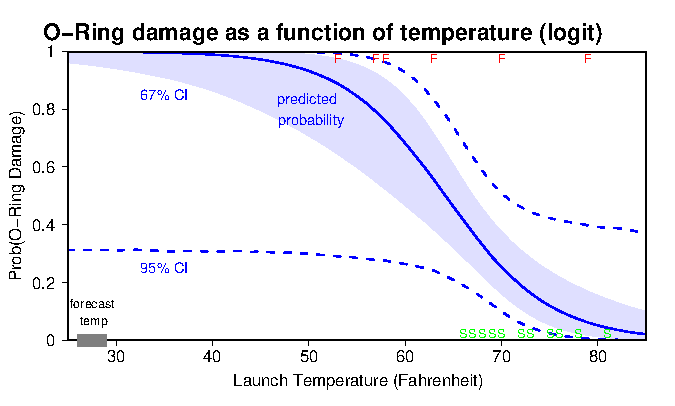
\includegraphics[width=10.5 in]{chall4}
\end{center}

Remembering that the Failures are only meaningful compared to Successes

\foilhead[-0.75in]{}

\color{black}
\begin{center}
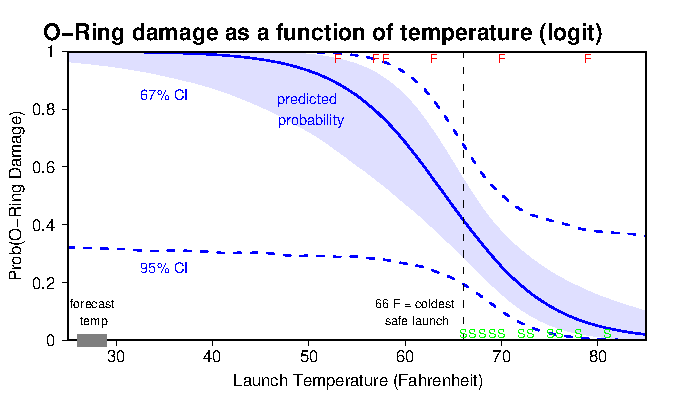
\includegraphics[width=10.5 in]{chall5}
\end{center}

\vspace{-2 em}

Looking just at the data tempts us to say that launches under 66 F are virtually guaranteed O-ring failures.  This inference is based on an unstated model.

\foilhead[-0.75in]{}

\color{black}
\begin{center}
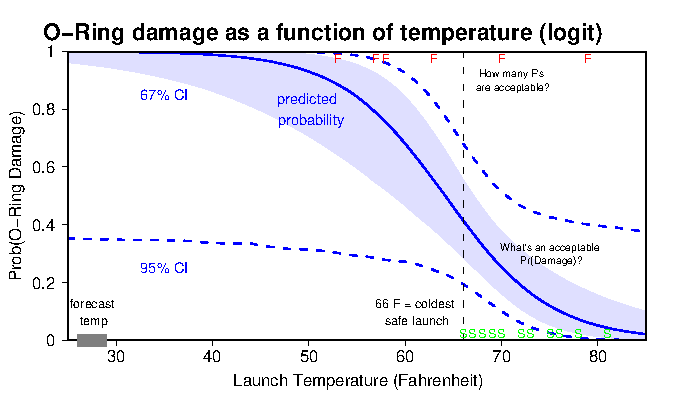
\includegraphics[width=10.5 in]{chall6}
\end{center}

\vspace{-2 em}

But the estimated logit model should give us pause.  

There is a significant risk of failure across the board.

\foilhead[-0.75in]{}

\color{black}
\begin{center}
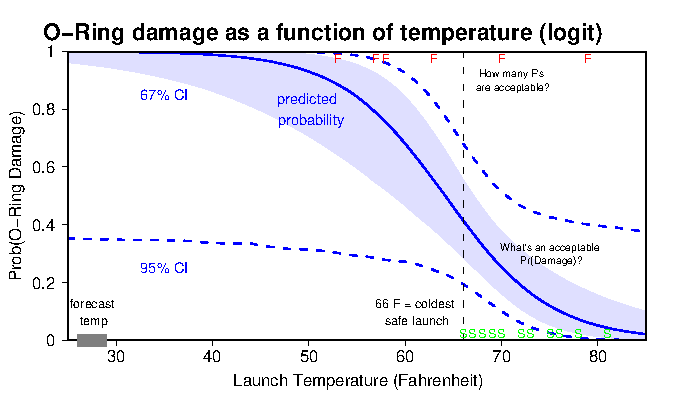
\includegraphics[width=10.5 in]{chall6}
\end{center}

\vspace{-2 em}

What is an acceptable risk of O-ring failure?  

Was the shuttle safe at any temperature?


\foilhead[-0.75in]{}
\bgclear

\vspace{-2 em}

\color{black}
\begin{center}
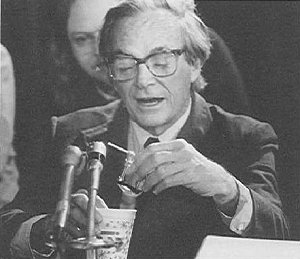
\includegraphics[width=4.5 in,angle=180]{feynnman}
\end{center}
\color{white}

In a hearing, Richard Feynmann dramatically showed O-rings lose resilence when cold\\
by dropping one in his ice water.

Experiment cut thru weeks of technical gibberish concealing flaws in the O-ring

But it shouldn't have taken a Nobel laureate: \\ 
any scientist with a year of statistical training could have \\
used the launch record to reach the same conclusion

And it would take no more than a single graphic to show the result


\foilhead[-0.75in]{Going further}
\bgclear

The Challenger example involves a simple, bivariate model

But even it goes beyond linear regression, because the outcome is binary, requiring a logit model

What else about these data might go beyond the simple linear regression framework?

\begin{itemize}
\item Serial correlation?  Perhaps wear from the last shuttle launch makes damage more likely in the next.

\item Panel structure?  Perhaps each rocket booster needs its own model
\end{itemize}

\foilhead[-0.75in]{Going further}
\bgclear

Social science data tend to be even more complicated:

Always many variables

Often interactive effects on responses

Serial correlation, heteroskedasticity, reverse causation, missing data, and more

In 503, we'll expand the linear model to cope with these problems and more

And prepare for future classes expanding your toolkit beyond linear modeling







\foilhead[-0.75in]{Why \texttt{R}?}
\bgclear

Real question:  Why programming?

\vspace{ 1 em}

Non-programmers stuck with package defaults

For your substantive problem, defaults may be 

\begin{itemize}
\item inappropriate (not quite the right model, but ``close'')

\item unintelligible (reams of non-linear coefficients and stars)
\end{itemize}

Programming allows you to match the methods to the data \& question

Get better, more easily explained results.

\foilhead[-0.75in]{Why \texttt{R}?}
\bgclear

Many side benefits:

\begin{enumerate}
\item Never forget what you did:  The code can be re-run.

\item Repeating an analysis $n$ times?  Write a loop!

\item Programming makes data processing/reshaping easy.

\item Programming makes replication easy.
\end{enumerate}

\foilhead[-0.75in]{Why \texttt{R}?}
\bgclear

\texttt{R} is 

\begin{itemize}
\item free

\item open source 

\item growing fast

\item widely used

\item the future for most fields
\end{itemize}

But once you learn one language, the others are much easier

\foilhead[-0.75in]{Introduction to R}
\bgclear

R is a calculator that can store lots of information in memory

R stores information as ``objects''

\begin{verbatim}
> x <- 2
> print(x)
[1] 2

> y <- "hello"
> print(y)
[1] "hello"

> z <- c(15, -3, 8.2)
> print(z)
[1] 15.0 -3.0  8.2
\end{verbatim}

\foilhead[-0.75in]{Introduction to R}
\bgclear

\begin{verbatim}
> w <- c("gdp", "pop", "income")
> print(w)
[1] "gdp"    "pop"    "income"
> 
\end{verbatim}

Note the assignment operator, \texttt{<-}, not \texttt{=}

An object in memory can be called to make new objects

\begin{verbatim}
> a <- x^2
> print(x)
[1] 2
> print(a)
[1] 4

> b <- z + 10
> print(z)
[1] 15.0 -3.0  8.2
> print(b)
[1] 25.0  7.0 18.2
\end{verbatim}

\foilhead[-0.75in]{Introduction to R}
\bgclear

\begin{verbatim}
> c <- c(w,y)
> print(w)
[1] "gdp"    "pop"    "income"
> print(y)
[1] "hello"
> print(c)
[1] "gdp"    "pop"    "income" "hello" 
\end{verbatim}

Commands (or ``functions'') in R are always written \texttt{command()}

The usual way to use a command is:

\begin{verbatim}
output <- command(input)
\end{verbatim}

We've already seen that \texttt{c()} pastes together variables.

A simple example:

\begin{verbatim}
> z <- c(15, -3, 8.2)
> mz <- mean(z)
> print(mz)
[1] 6.733333
\end{verbatim}

\foilhead[-0.75in]{Introduction to R}
\bgclear

Some commands have multiple inputs.  Separate them by commas:

\texttt{plot(var1,var2)}  plots var1 against var2

Some commands have optional inputs.  If omitted, they have default values.

\texttt{plot(var1)} plots var1 against the sequence \{1,2,3,\ldots\}

Inputs can be identified by their position or by name.

\texttt{plot(x=var1,y=var2)} plots  var2 against var1


\foilhead[-0.75in]{Entering code}
\bgclear

You can enter code by typing at the prompt, by cutting or pasting, or from a file

If you haven't closed the parenthesis, and hit enter, \texttt{R} let's you continue with this prompt \texttt{+}

You can copy and paste multiple commands at once

You can run a text file containing a program using \texttt{source()}, with the name of the file as input (ie, in "")

I prefer the \texttt{source()} approach.  Leads to good habits of retaining code.



\foilhead[-0.75in]{Data types}

R has three important data types to learn now

\begin{tabular}{ll}
Numeric  &  \texttt{y <- 4.3} \\
Character   &  \texttt{y <- "hello"} \\
Logical  &  \texttt{y <- TRUE}
\end{tabular}

We can always check a variable's type, and sometimes change it:

\begin{verbatim}
population <- c("1276", "562", "8903")
print(population)
is.numeric(population)
is.character(population)
\end{verbatim}

Oops!  The data have been read in as characters, or ``strings''.  R does not know they are numbers.

\begin{verbatim}
population <- as.numeric(population)
\end{verbatim}

\foilhead[-0.75in]{Some special values}

\begin{tabular}{ll}
Missing data &   \texttt{NA} \\
A ``blank''  &   \texttt{NULL} \\
Infinity     &   \texttt{Inf} \\
Not a number &   \texttt{NaN} \\
\end{tabular}

\foilhead[-0.75in]{Data structures}

All R objects have a data type \emph{and} a data structure

Data structures can contain numeric, character, or logical entries

Important structures:

\begin{center}
Vector 

Matrix 

Dataframe 

List (to be covered later)
\end{center}

\foilhead[-0.75in]{Vectors in R}

Vector is R are simply 1-dimensional lists of numbers or strings

Let's make a vector of random numbers:

\begin{verbatim}
x <- rnorm(1000)
\end{verbatim}

x contains 1000 random normal variates drawn from a Normal
distribution with mean 0 and standard deviation 1.

What if we wanted the mean of this vector?

\begin{verbatim}
mean(x)
\end{verbatim}

What if we wanted the standard deviation?

\begin{verbatim}
sd(x)
\end{verbatim}

\foilhead[-0.75in]{Vectors in R}

What if we wanted just the first element?

\begin{verbatim}
x[1]
\end{verbatim}

or the 10th through 20th elements?

\begin{verbatim}
x[10:20]
\end{verbatim}

what if we wanted the 10th percentile?

\begin{verbatim}
sort(x)[100]
\end{verbatim}

Indexing a vector can be very powerful.  Can apply to any vector object.

What if we want a histogram?

\begin{verbatim}
hist(x)
\end{verbatim}

\foilhead[-0.75in]{Vectors in R}

Useful commands for vectors:

\begin{tabular}{ll}
\texttt{seq(from, to, by)} &generates a sequence\\

\texttt{rep(x,times)} &repeats \texttt{x} \\

\texttt{sort()} &sorts a vector from least to greatest\\
  
\texttt{rev()} &reverses the order of a vector\\

\texttt{rev(sort())} &sorts a vector from greatest to least\\
\end{tabular}



\foilhead[-0.75in]{Matrices in R}

Vector are the standard way to store and manipulate variables in R

But usually our datasets have several variables measured on the same observations

Several variables collected together form a matrix with one row for each observation and one column for each variable

\foilhead[-0.75in]{Matrices in R}

Many ways to make a matrix in R

\begin{verbatim}
a <- matrix(data=NA, nrow, ncol, byrow=FALSE)
\end{verbatim}

This makes a matrix of \texttt{nrow} $\times$ \texttt{ncol}, and fills it with missing values.

To fill it with data, substitute a vector of data for NA in the command.  It will fill up the matrix column by column.

We could also paste together vectors, binding them by column or by row:

\begin{verbatim}
b <- cbind(var1, var2, var3)
c <- rbind(obs1, obs2)
\end{verbatim}

\foilhead[-0.75in]{Matrices in R}

Optionally, R can remember names of the rows and columns of a matrix

To assign names, use the commands:

\begin{verbatim}
colnames(a) <- c("Var1", "Var2")
rownames(a) <- c("Case1", "Case2")
\end{verbatim}

Substituting the actual names of your variables and observations (and making sure there is one name for each variable \& observation)

\foilhead[-0.75in]{Matrices in R}

Matrices are indexed by row and column.

We can subset matrices into vectors or smaller matrices

\begin{tabular}{ll}
\texttt{a[1,1]}      &  Gets the first element of a \\
\texttt{a[1:10,1]}   &  Gets the first ten rows of the first column \\
\texttt{a[,5]}       &  Gets every row of the fifth column \\
\texttt{a[4:6,]}     &  Gets every column of the 4th through 6th rows \\
\end{tabular}

To make a vector into a matrix, use \texttt{as.matrix()}

R defaults to treating one-dimensional arrays as vectors, not matrices


Useful matrix commands:

\begin{tabular}{ll}
\texttt{nrow()}    &Gives the number of rows of the matrix\\

\texttt{ncol()}    &Gives the number of columns\\

\texttt{t()}       &Transposes the matrix\\
\end{tabular}

Much more on matrices next week.

\foilhead[-0.75in]{Dataframes in R}

Dataframes are a special kind of matrix used to store datasets

To turn a matrix into a dataframe (note the extra .):

\begin{verbatim}
a <- as.data.frame(a)
\end{verbatim}

Dataframes always have columns names, and these are set or retrieved using the \texttt{names()} command

\begin{verbatim}
names(a) <- c("Var1","Var2")
\end{verbatim}

Dataframes can be ``attached'', which makes each column into a vector with the appropriate name

\begin{verbatim}
attach(a)
\end{verbatim}


\foilhead[-0.75in]{Loading data}

There are many ways to load data to R.  I prefer using comma-separated variable files, which can be loaded with \texttt{read.csv}

You can also check the \texttt{foreign} library for other data file types

If your data have variable names, you can attach the dataset like so:

\begin{verbatim}
data <- read.csv("mydata.csv")
attach(data)
\end{verbatim}

to access the variables directly


\foilhead[-0.75in]{Benefits and dangers of \texttt{attach()}}


If your data have variable names, you can also ``attach'' the dataset like so:

\begin{verbatim}
data <- read.csv("mydata.csv")
attach(data)
\end{verbatim}

to access all the variables directly through newly created vectors.


\emph{Be careful!}  \texttt{attach()} is tricky.

\begin{enumerate}
\item If you attach a variable \texttt{data\$x} in \texttt{data} and
  then modify \texttt{x}, the original \texttt{data\$x} is unchanged.

\item  If you have more than one dataset with the same variable names,
  \texttt{attach()} is a bad idea:  only the first will be attached!

\end{enumerate}

Sometimes \texttt{attach()} is handy, but be careful!


\foilhead[-0.75in]{Missing data}

When loading a dataset, you can often tell R what symbol that file uses for missing data using the option \texttt{na.strings=}

So if your dataset codes missings as ., set \texttt{na.strings="."}

If your dataset codes missings as a blank, set \texttt{na.strings=""}

If your dataset codes missings in multiple ways, you could set, e.g., \texttt{na.strings=c(".","","NA")}

\foilhead[-0.75in]{Missing data}

Many R commands will not work properly on vectors, matrices, or dataframes containing missing data (NAs)

To check if a variables contains missings, use \texttt{is.na(x)}

To create a new variable with missings listwise deleted, use \texttt{na.omit}

If we have a dataset \texttt{data} with NAs at data[15,5] and data[17,3]

\begin{verbatim}
dataomitted <- na.omit(data)
\end{verbatim}
will create a new dataset with the 15th and 17th rows left out

Be careful!  If you have a variable with lots of NAs you are not using in your analysis, remove it from the dataset \emph{before} using \texttt{na.omit()}

\foilhead[-0.75in]{Mathematical Operations}

\texttt{R} can do all the basic math you need

Binary operators:  \begin{verbatim} + - * / ^ \end{verbatim}

Binary comparisions:  \begin{verbatim}  < <= > >= == != \end{verbatim}

Logical operators (and, or, and not; use
parentheses!):  \begin{verbatim}  & | ! && || \end{verbatim}

Math/stat fns:  \begin{verbatim} log exp mean median min max sd var cov cor \end{verbatim}

Set functions (see \texttt{help(sets)}), Trigonometry (see \texttt{help(Trig)}), 

\texttt{R} follows the usual order of operations; if it doubt, use parentheses


\foilhead[-0.75in]{Example 1:  US Economic growth}

Let's investigate an old question in political economy:

Are there partisan cycles, or tendencies, in economic performance?

Does one party tend to produce higher growth on average?

(Theory:  Left cares more about growth vis-a-vis inflation than the Right

If there is partisan control of the economy, \\
then Left should have higher growth ceteris paribus)

Data from the Penn World Tables (Annual growth rate of GDP in percent)

Two variables:

\begin{tabular}{ll}
\texttt{grgdpch}   &The per capita GDP growth rate \\
\texttt{party}     &The party of the president (Dem =  -1, Rep = 1) \\
\end{tabular}

\foilhead[-0.75in]{Example 1:  US Economic growth}

\begin{verbatim}
# Load data
data <- read.csv("gdp.csv",na.strings="")
attach(data)

# Construct party specific variables
gdp.dem <- grgdpch[party==-1]
gdp.rep <- grgdpch[party==1]

# Make the histogram
hist(grgdpch,
     breaks=seq(-5,8,1),
     main="Histogram of US GDP Growth, 1951--2000",
     xlab="GDP Growth")

\end{verbatim}


\foilhead[-0.75in]{}
\bgclear
\bgadd{\vspace{0 in} \\ 
\includegraphics[width=12 in,height=9 in]{whiteback.jpg}}

\begin{center}
\color{black}
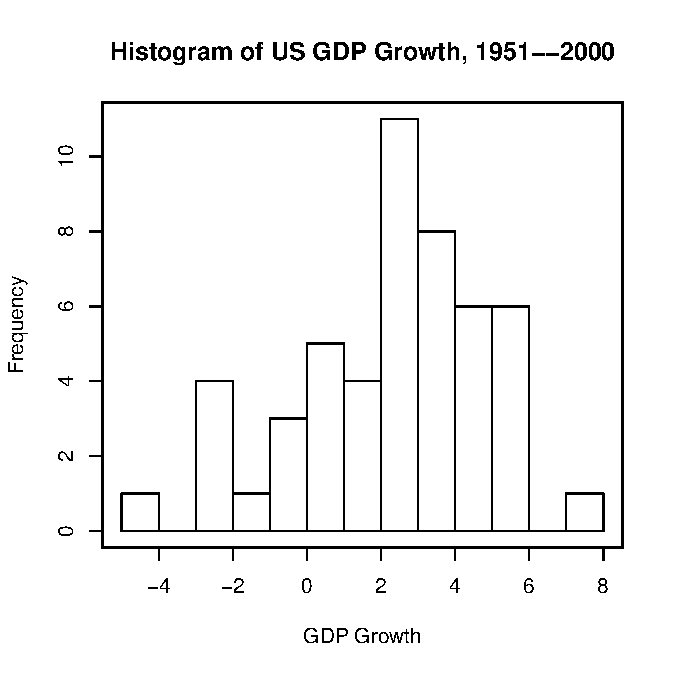
\includegraphics[width=7.5 in]{gdphist_all}
\color{white}
\end{center}

\foilhead[-0.75in]{}
\bgclear
\bgadd{\vspace{0 in} \\ 
\includegraphics[width=12 in,height=9 in]{whiteback.jpg}}

\begin{center}
\color{black}
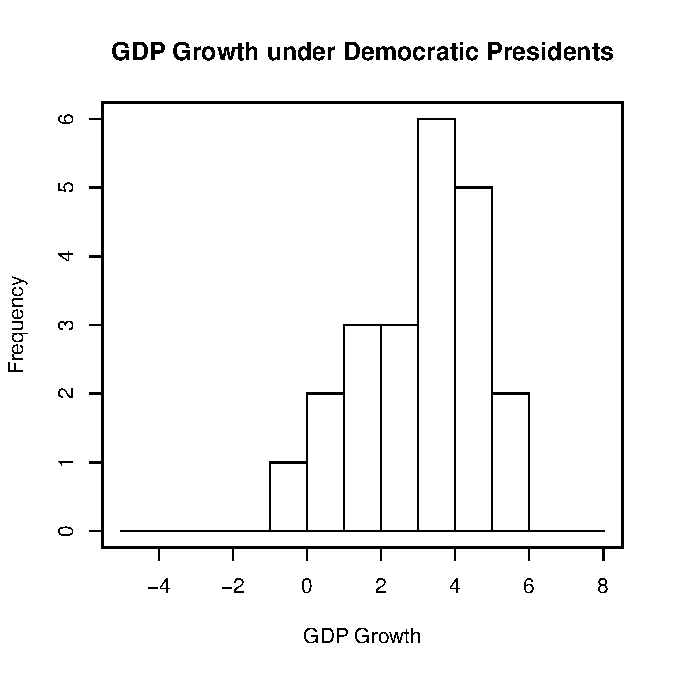
\includegraphics[width=7.5 in]{gdphist_dem}
\color{white}
\end{center}


\foilhead[-0.75in]{}
\bgclear
\bgadd{\vspace{0 in} \\ 
\includegraphics[width=12 in,height=9 in]{whiteback.jpg}}

\begin{center}
\color{black}
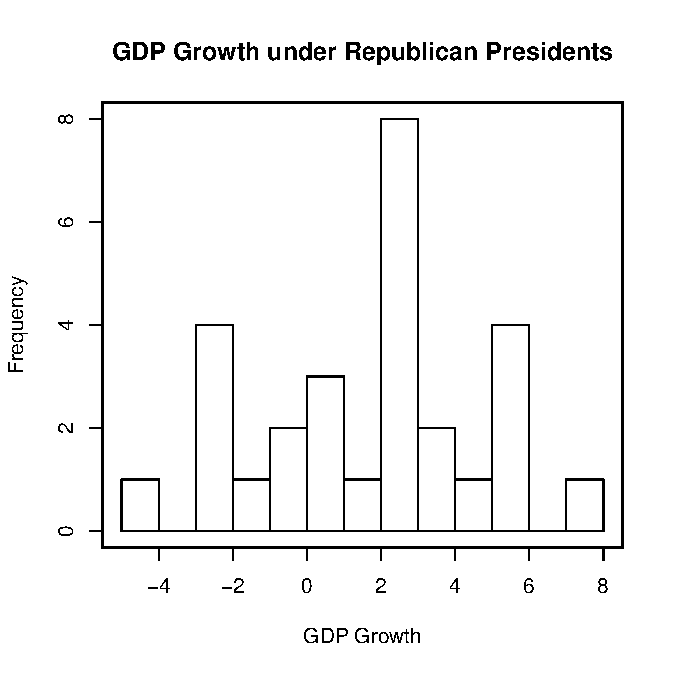
\includegraphics[width=7.5 in]{gdphist_rep}
\color{white}
\end{center}

\foilhead[-0.75in]{}
\bgclear

\begin{verbatim}
# Make a box plot
boxplot(grgdpch~as.factor(party),
        boxwex=0.3,
        range=0.5,
        names=c("Democratic\n Presidents",
          "Republican\n Presidents"),
        ylab="GDP growth",
        main="Economic performance of partisan governments")
\end{verbatim}

Note the unusual first input:  this is an R formula
\begin{verbatim}
y~x1+x2+x3
\end{verbatim}

In this case, \texttt{grgdpch} is being ``modelled'' as a function of \texttt{party}

\texttt{boxplot()} needs party to be a ``factor'' or an explicitly categorical variable

Hence we pass boxplot \texttt{as.factor(party)}, which turns the numeric variable into a factor


\foilhead[-0.75in]{Box plots:  Annual US GDP growth, 1951--2000}
\bgclear
\bgadd{\vspace{1.9 in} \\ 
\includegraphics[width=12 in,height=9 in]{whiteback.jpg}}

\begin{center}
\color{black}
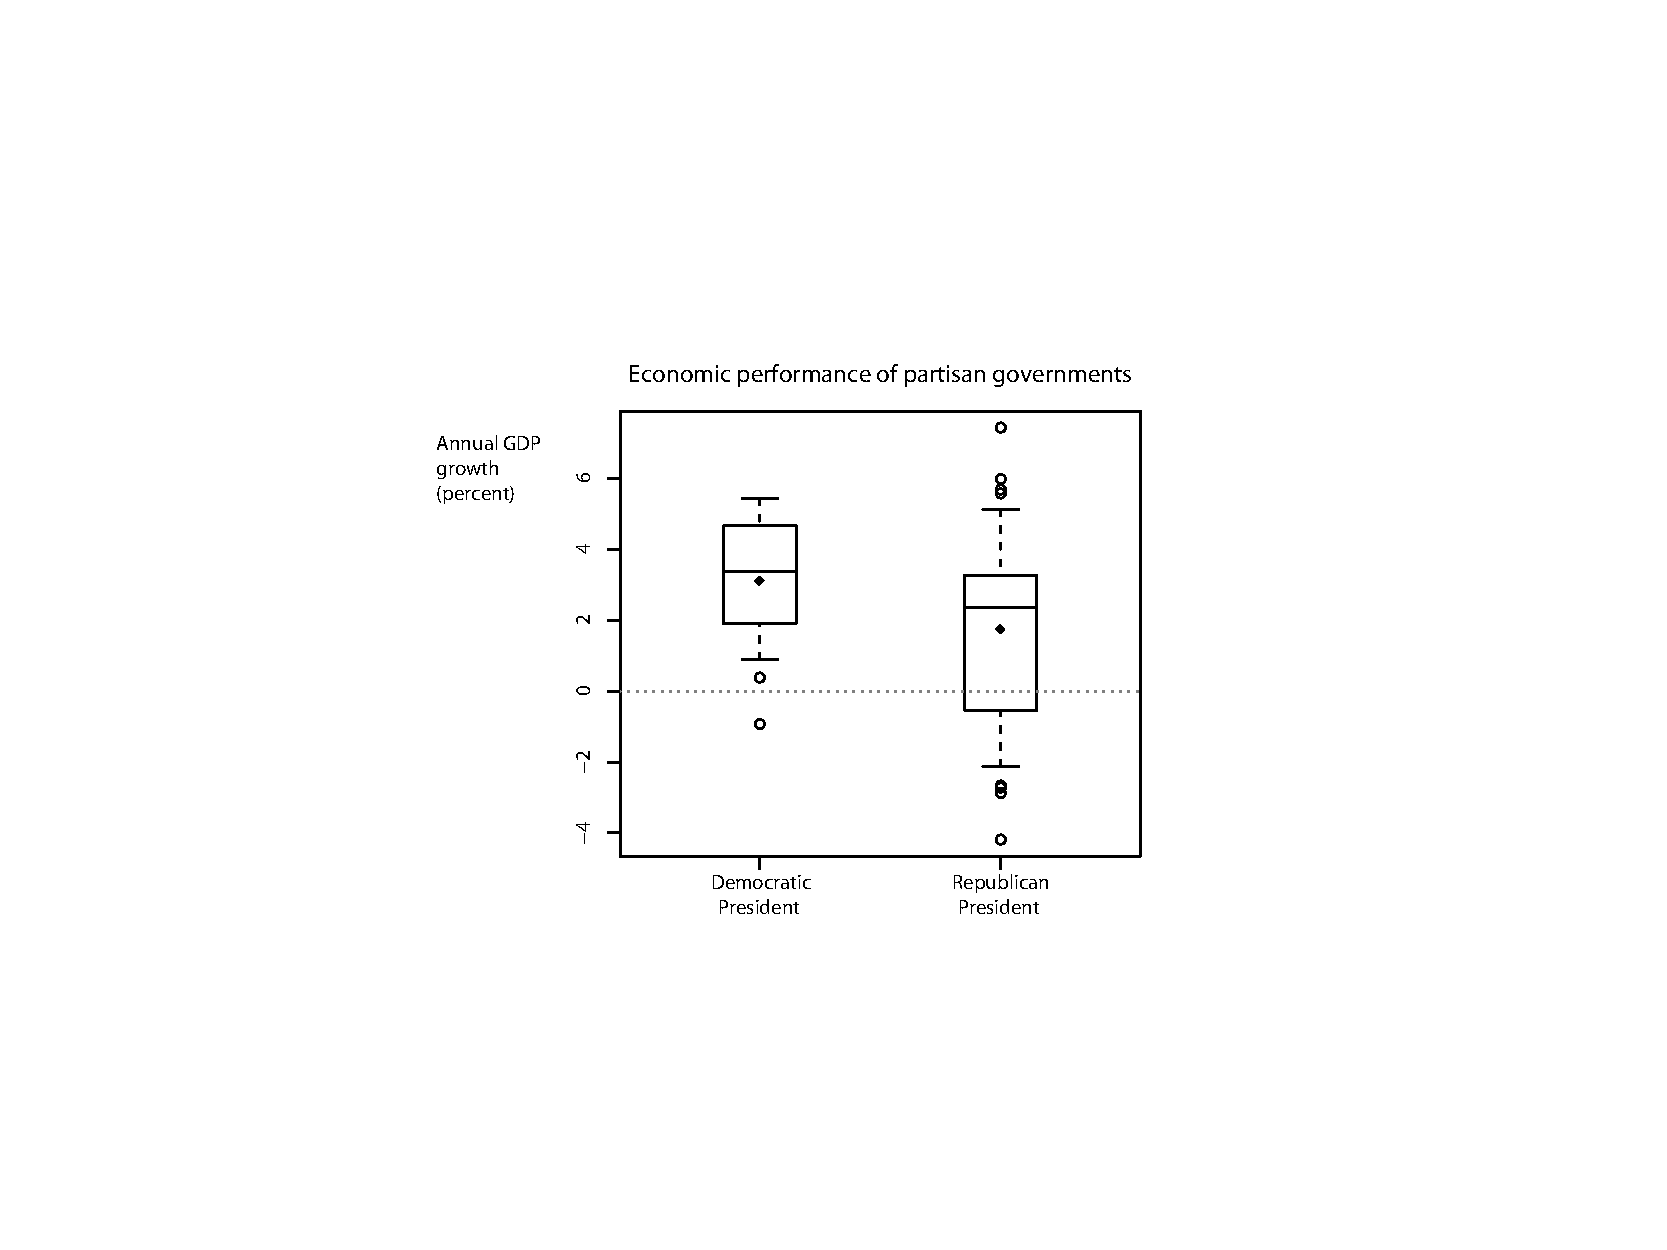
\includegraphics[width=9 in]{gdpbox1}
\color{white}
\end{center}

\foilhead[-0.75in]{Box plots:  Annual US GDP growth, 1951--2000}
\bgclear
\bgadd{\vspace{1.9 in} \\ 
\includegraphics[width=12 in,height=9 in]{whiteback.jpg}}

\begin{center}
\color{black}
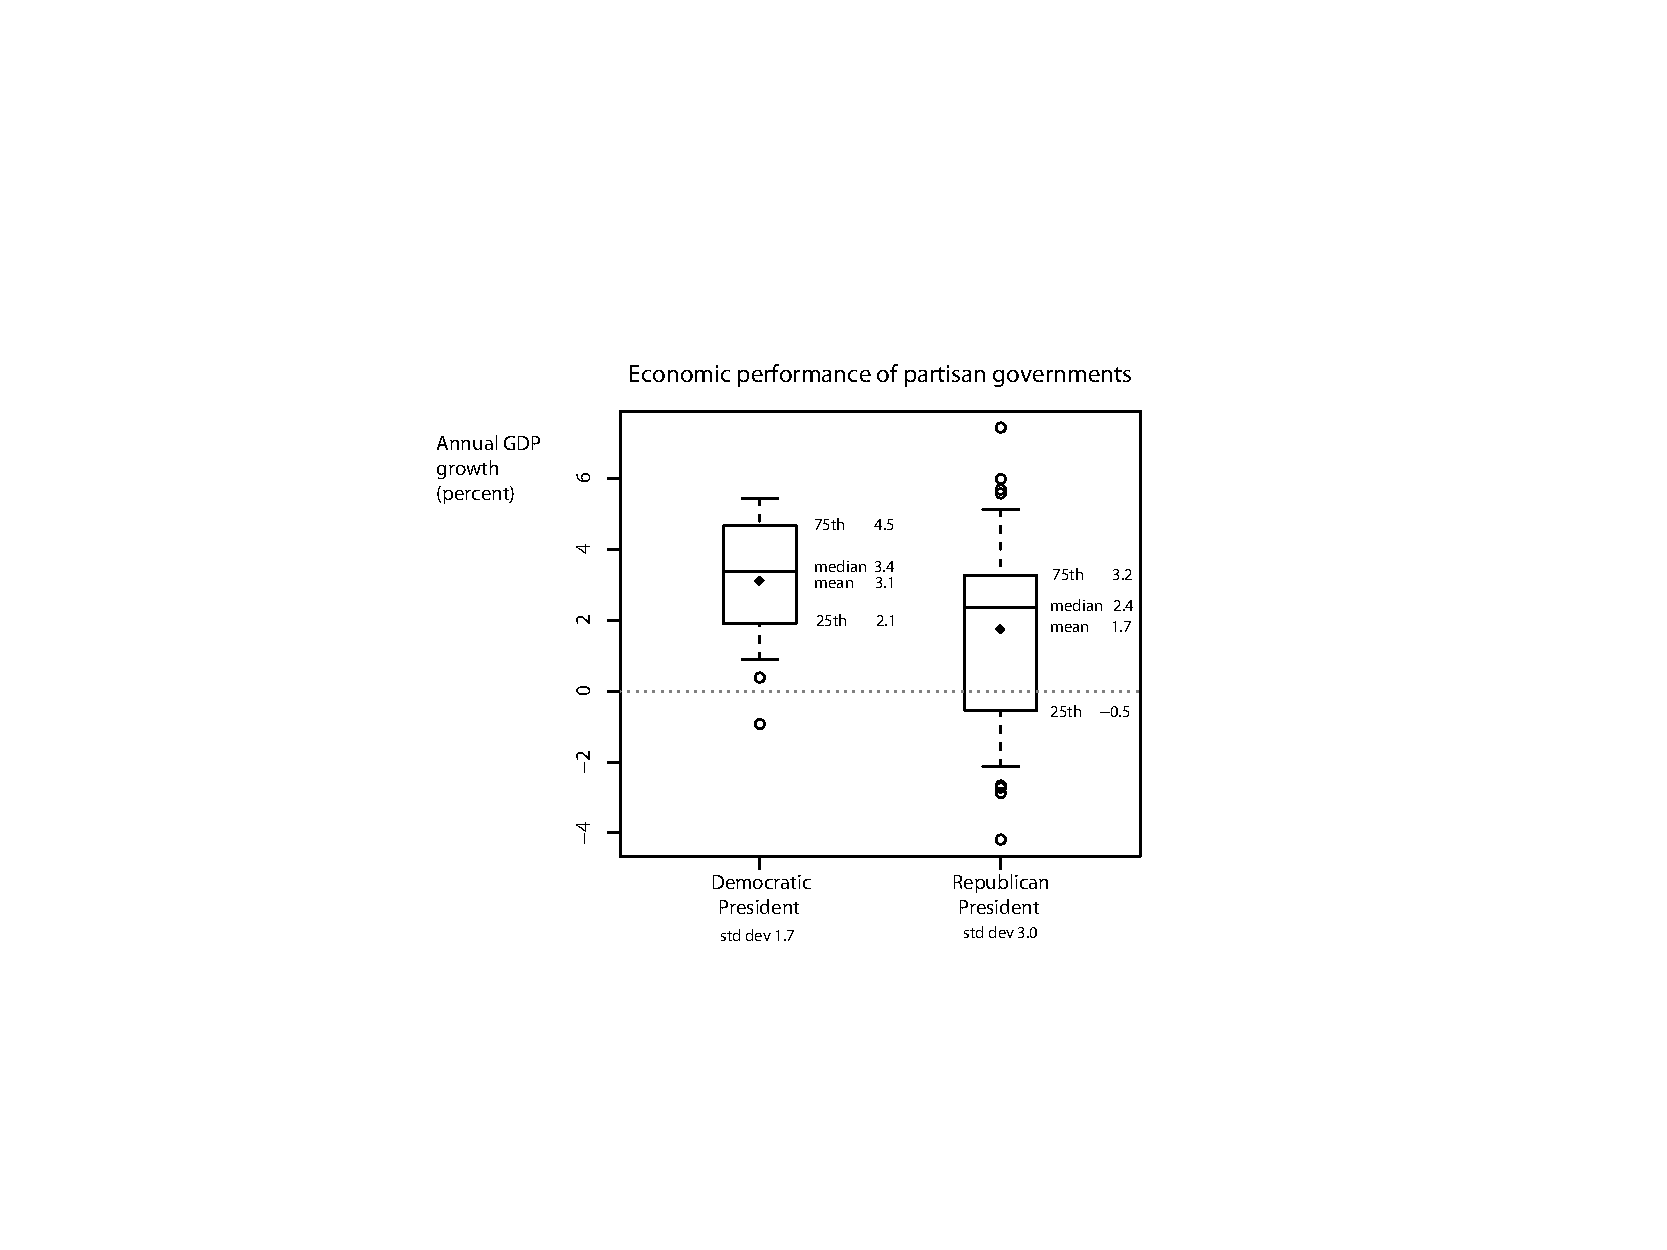
\includegraphics[width=9 in]{gdpbox2}
\color{white}
\end{center}

\foilhead[-0.75in]{Box plots:  Annual US GDP growth, 1951--2000}
\bgclear
\bgadd{\vspace{1.9 in} \\ 
\includegraphics[width=12 in,height=9 in]{whiteback.jpg}}

\begin{center}
\color{black}
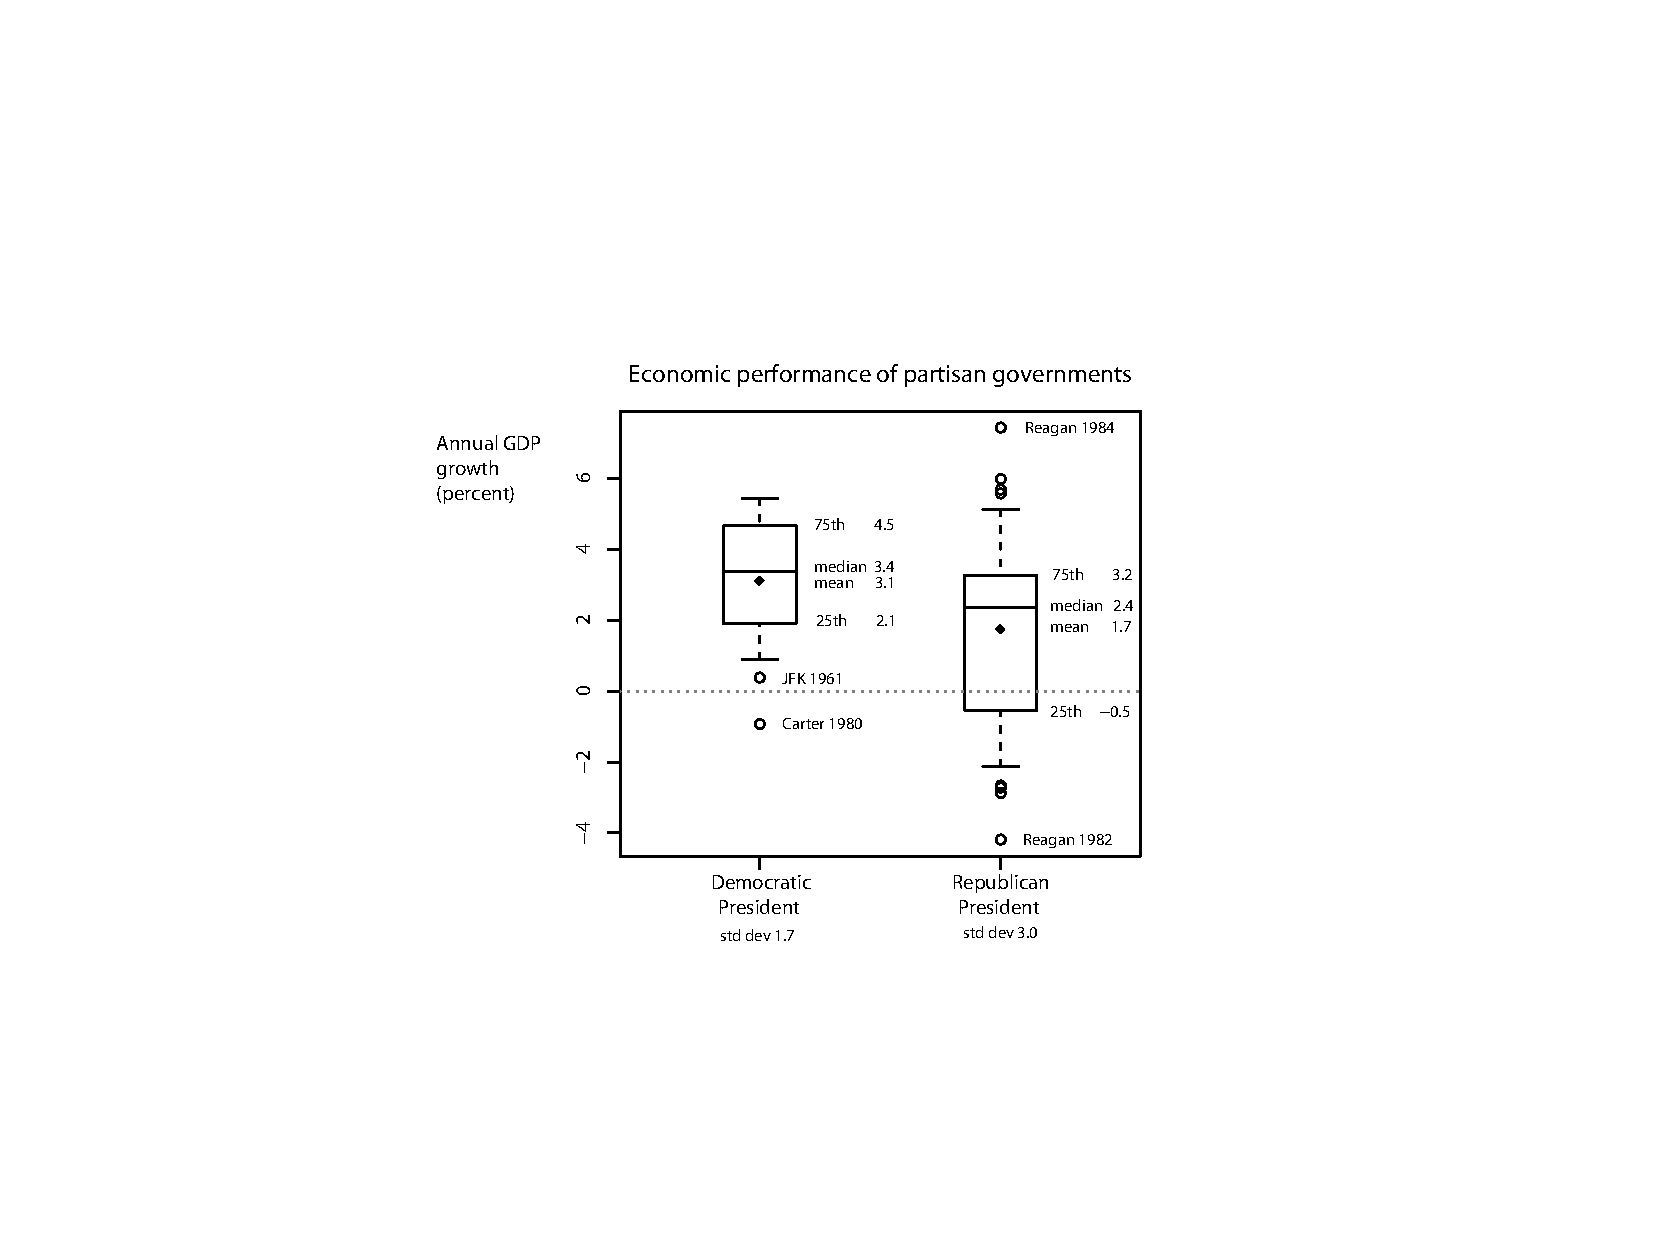
\includegraphics[width=9 in]{gdpbox4}
\color{white}
\end{center}

\foilhead[-0.75in]{Box plots:  Annual US GDP growth, 1951--2000}
\bgclear
\bgadd{\vspace{1.9 in} \\ 
\includegraphics[width=12 in,height=9 in]{whiteback.jpg}}

\begin{center}
\color{black}
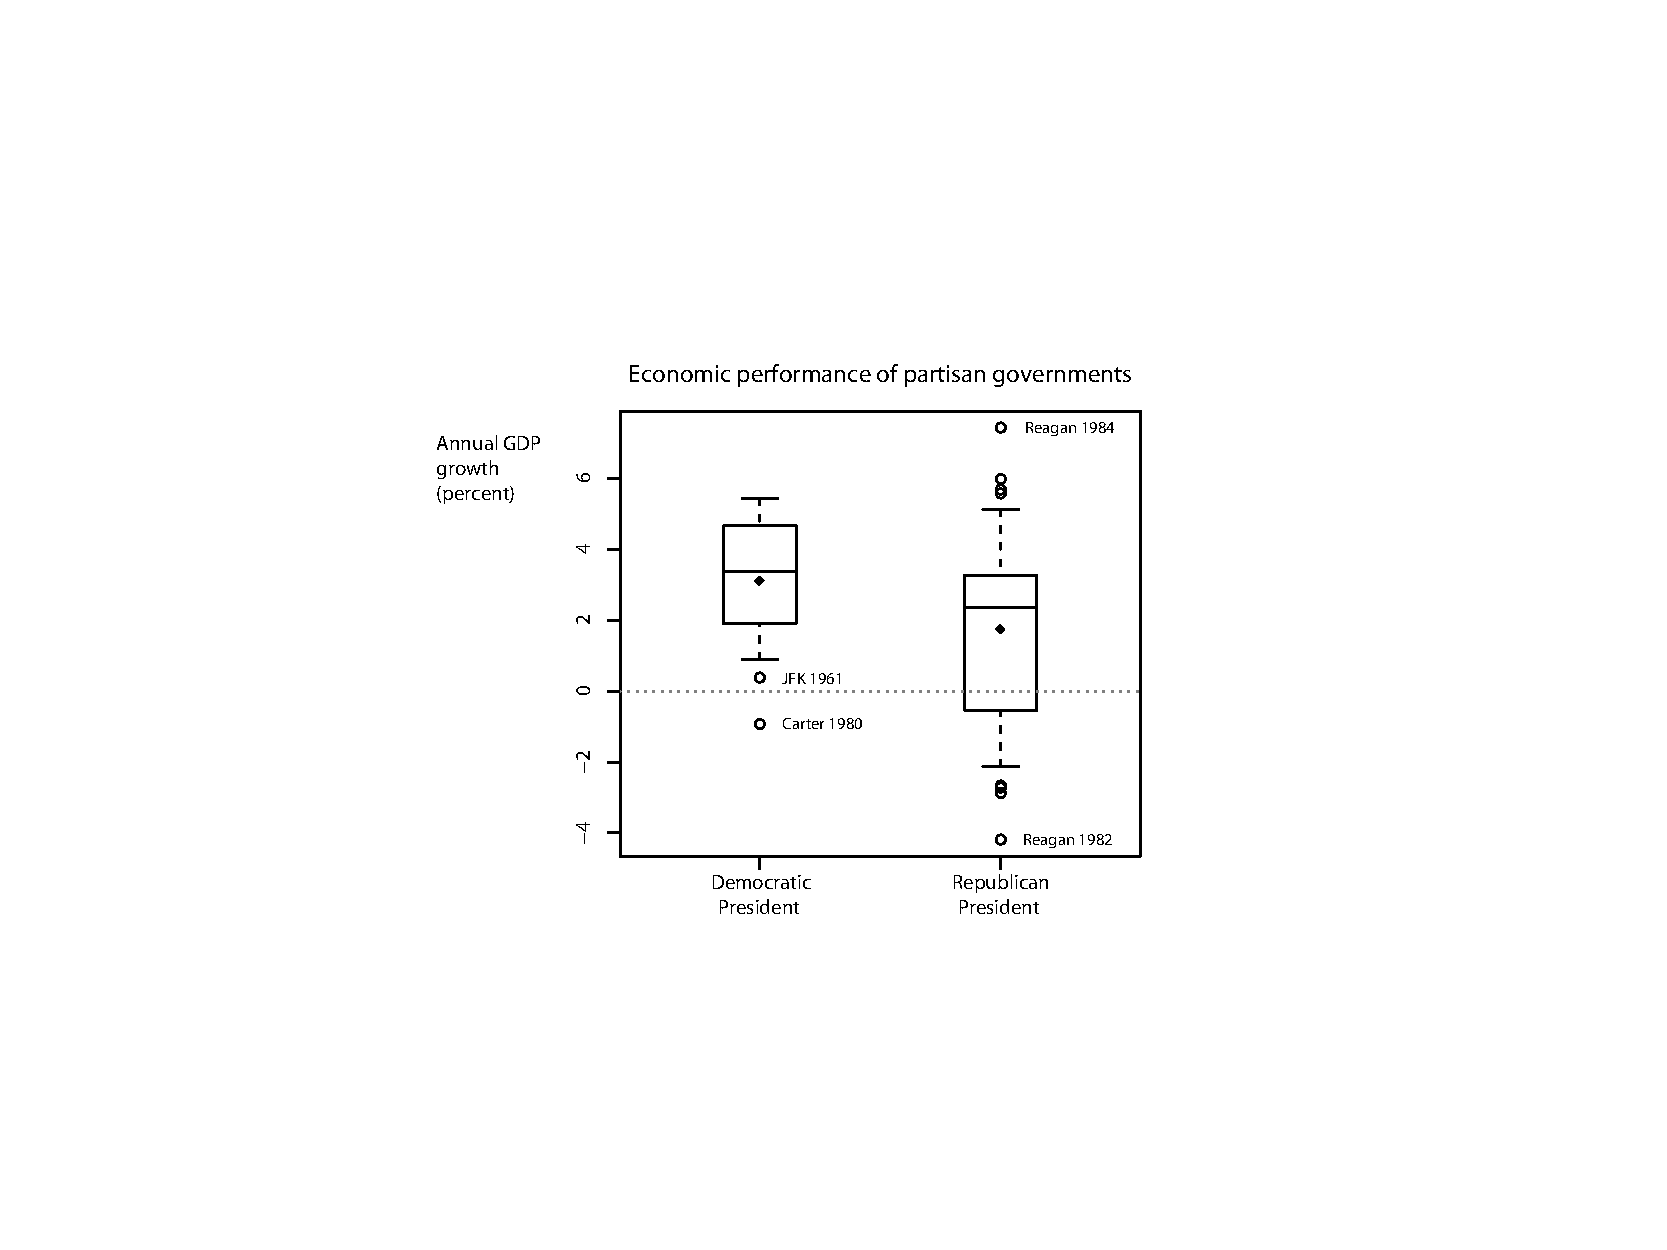
\includegraphics[width=9 in]{gdpbox3}
\color{white}
\end{center}



\foilhead[-0.75in]{Help!}
\bgclear

To get help on a known command \texttt{x}, type \texttt{help(x)} or \texttt{?x}

To search the help files using a keyword string \texttt{s}, type \texttt{help.search(s)} 

Note that this implies to search on the word regression, you should type\\
\texttt{help.search("regression")} 

but to get help for the command \texttt{lm}, you should type
\texttt{help(lm)} 


\foilhead[-0.75in]{Installing R on a PC}
\bgclear

\begin{itemize}
\item Go to the Comprehensive R Archive Network (CRAN) \\
      \texttt{http://cran.r-project.org/}

\item Under the heading ``Download and Install R'', click on ``Windows''

\item Click on ``base''

\item Download and run the R setup program.  \\
The name changes as R gets updated; \\
the current version is ``R-2.14.2-win.exe''

\item Once you have R running on your computer, \\
you can add new libraries from inside R by selecting \\
``Install packages'' from the Packages menu
\end{itemize}

\foilhead[-0.75in]{Installing R on a Mac}
\bgclear

\begin{itemize}
\item Go to the Comprehensive R Archive Network (CRAN) \\
      \texttt{http://cran.r-project.org/}

\item Under the heading ``Download and Install R'', click on ``MacOS X''

\item Download and run the R setup program.  \\
The name changes as R gets updated; \\
the current version is ``R-2.14.2.pkg''

\item Once you have R running on your computer, \\
you can add new libraries from inside R by selecting \\
``Install packages'' from the Packages menu
\end{itemize}

\foilhead[-0.75in]{Editing scripts}
\bgclear

Don't use Microsoft Word to edit R code!

Word adds lots of ``stuff'' to text; R needs the script in a plain text file.

Some text editors:

\begin{itemize}
\item \textbf{Notepad:}  Free, and comes with Windows (under Start
  $\rightarrow$ Programs $\rightarrow$ Accessories).  Gets the job
  done; not powerful.

\item \textbf{TextEdit:}  Free, and comes with Mac OS X.  Gets the job done;
  not powerful.

\item \textbf{TINN-R:}  Free and fairly powerful.  Windows only.\\
\texttt{http://www.sciviews.org/Tinn-R/}

\item \textbf{Emacs:} Free and very powerful (my preference).  Can use
  for R and Latex.  Available
  for Mac and PC.\\

For Mac (easy installation):  \texttt{http://aquamacs.org/}

For Windows (see the README):  \texttt{http://ftp.gnu.org/gnu/emacs/windows/}



\end{itemize}

\foilhead[-0.75in]{Editing data}
\bgclear

R can load many other packages' data files

See the \texttt{foreign} library for commands

For simplicity \& universality, I prefer Comma-Separated Variable (CSV) files

Microsoft Excel can edit and export CSV files (under Save As)

R can read them using \texttt{read.csv()}

OpenOffice is free alternative to Excel \& makes CSV files (for all platforms): \\
\texttt{http://www.openoffice.org/}

\bigskip

\bigskip

\bigskip

My detailed guide to installing social science
software on the Mac:  \texttt{http://thewastebook.com/?post=social-science-computing-for-mac}

Focus on steps 1.1 and 1.3 for now; come back later for Latex in step 1.2

\foilhead[-0.75in]{Example 2: A simple linear regression}
\bgclear

Let's investigate a bivariate relationship

Cross-national data on fertility (children born per adult female) and the percentage of women practicing contraception.

Data are from 50 developing countries.

Source: Robey, B., Shea, M. A., Rutstein, O. and Morris, L. (1992)
``The reproductive revolution: New survey findings.''
\emph{Population Reports.} Technical Report M-11.

\foilhead[-0.75in]{Example 2: A simple linear regression}
\bgclear

\begin{verbatim}
# Load data
data <- read.csv("robeymore.csv",header=T,na.strings="")
completedata <- na.omit(data)
attach(completedata)

# Transform variables
contraceptors <- contraceptors/100

# Run linear regression
res.lm <- lm(tfr~contraceptors)
print(summary(res.lm))

# Get predicted values
pred.lm <- predict(res.lm)
\end{verbatim}

\foilhead[-0.75in]{Example 2: A simple linear regression}
\bgclear

\begin{verbatim}
# Make a plot of the data
plot(x=contraceptors,
     y=tfr,
     ylab="Fertility Rate",
     xlab="% of women using contraception",
     main="Average fertility rates & contraception; \n
           50 developing countries",
     xaxp=c(0,1,5)
     )

# Add predicted values to the plot
points(x=contraceptors,y=pred.lm,pch=16,col="red") 
\end{verbatim}

\foilhead[-0.75in]{Example 2: A simple linear regression}
\bgclear

\begin{verbatim}
> summary(res.lm)

Call:
lm(formula = tfr ~ contraceptors)

Residuals:
     Min       1Q   Median       3Q      Max 
-1.54934 -0.30133  0.02540  0.39570  1.20214 

Coefficients:
              Estimate Std. Error t value Pr(>|t|)    
(Intercept)     6.8751     0.1569   43.83   <2e-16 ***
contraceptors  -5.8416     0.3584  -16.30   <2e-16 ***
---
Signif. codes:  0 `***' 0.001 `**' 0.01 `*' 0.05 `.' 0.1 ` ' 1 

Residual standard error: 0.5745 on 48 degrees of freedom
Multiple R-Squared: 0.847,      Adjusted R-squared: 0.8438 
F-statistic: 265.7 on 1 and 48 DF,  p-value: < 2.2e-16 
\end{verbatim}

\foilhead[-0.75in]{Data and Prediction}
\bgclear
\bgadd{\vspace{1.75 in} \\ 
\includegraphics[width=12 in,height=6.15 in]{whiteback.jpg}}

\begin{center}
\color{black}
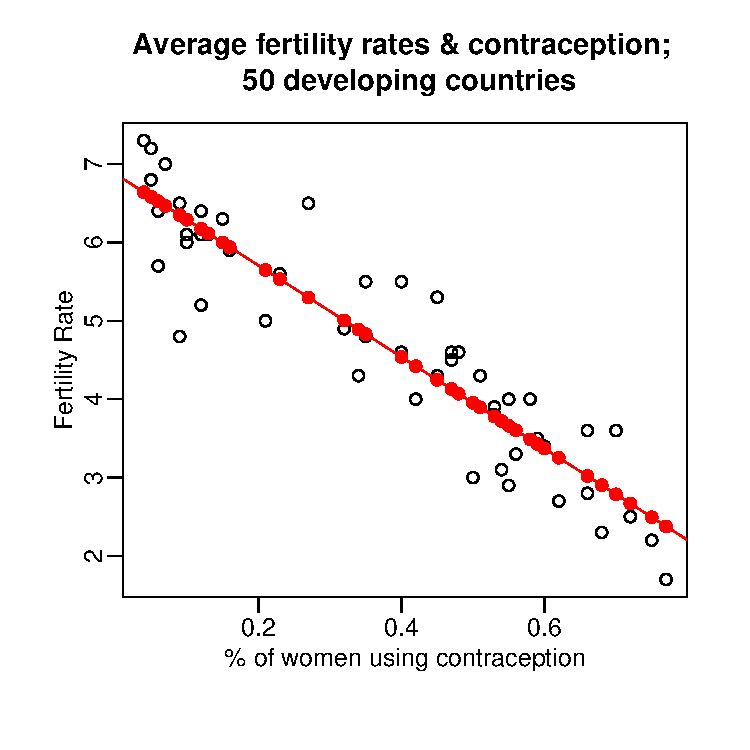
\includegraphics[width=6.7 in]{predictedfert1}
\color{white}
\end{center}

\end{document}
